\AntoineSpeak
\subsection{Intégration}
\begin{frame}{Intégration\ldots}
\begin{figure}
	\centering
	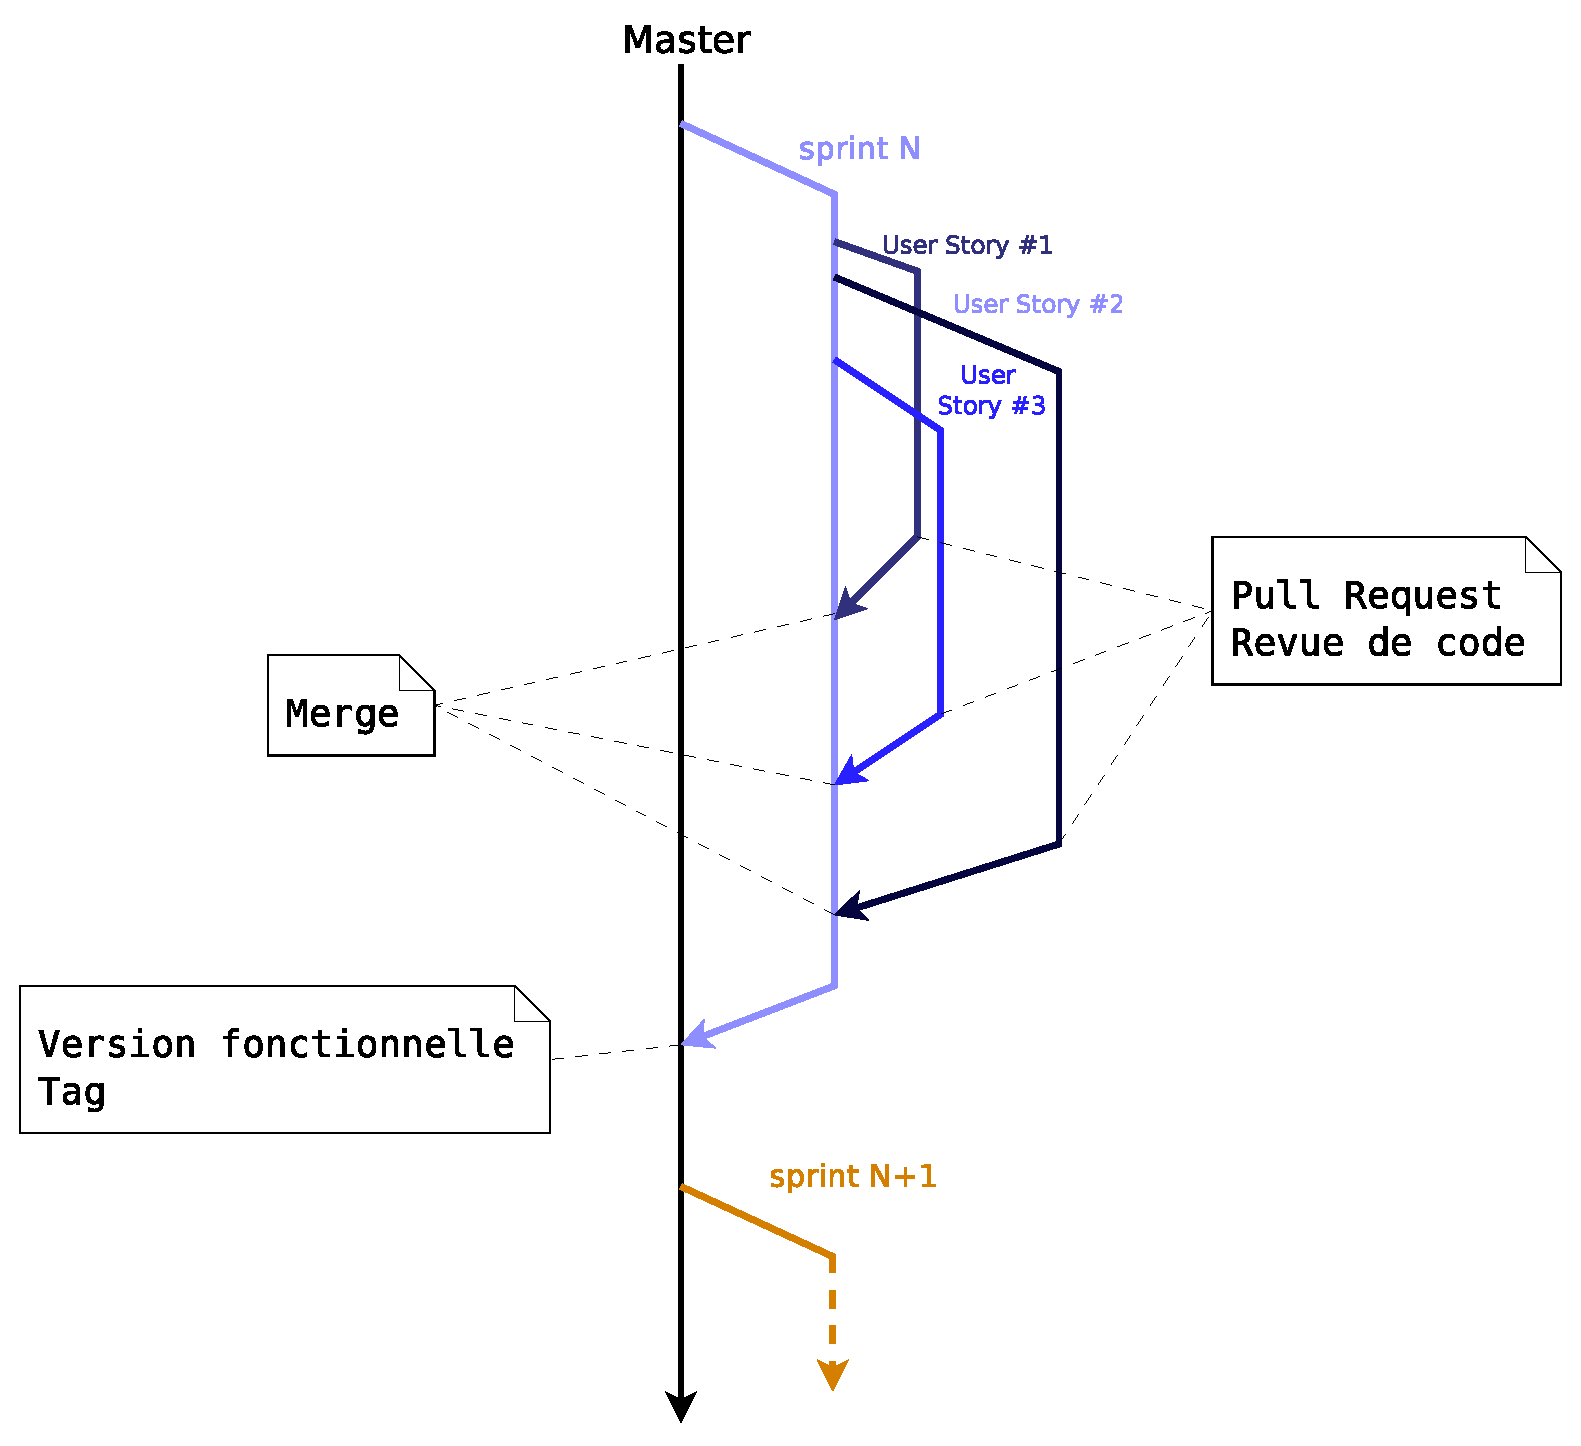
\includegraphics[width=0.83\linewidth]{images/Process/BranchingWorkflow}
	\caption{Git \textit{feature branch workflow}}
	\label{fig:BranchingWorkflow}
\end{figure}
\end{frame}
\begin{frame}{\ldots Continue}	
	\vfill
	Utilisation de \texttt{Travis-CI} : 
\begin{itemize}
	\item Tâches exécutées à chaque \textit{push} :
		\begin{itemize}
			\item Compilation du projet
			\item Exécution des tests unitaires
			\item Exécution des tests d'intégration
			\item Calcul de la couverture de code
			\item Déploiement de master sur Heroku
		\end{itemize}
\end{itemize}
\vfill
\centering
$\Longrightarrow$ Si tout est bon 
\includegraphics[width=1.2cm]{images/build}
\end{frame}
\ZacSpeak
\subsection{Vérification}
\begin{frame}{Vérification}
	\begin{itemize}
		\item Tests unitaires avec \texttt{Spock} pour : 
		\begin{itemize}
			\item Les classes de modèles
			\item Les contrôleurs
			\item Les services (hors DAO)
		\end{itemize}
		\vfill
		\item Calcul du taux de couverture avec \texttt{Cobertura} 
		\begin{itemize}
			\item Objectif de 80\% par ligne de code
		\end{itemize}
				\vfill
		\item Tableau de bord du projet à l'aide de \texttt{SonarQube}
		\begin{itemize}
			\item Couverture, documentation, commentaires, \ldots 
			\item Complexité de code
		\end{itemize}
				\vfill
		\item \texttt{Codenarc} pour l'analyse statique 
		\begin{itemize}
			\item Convention de codage standard Groovy
		\end{itemize}
	\end{itemize}
\end{frame}

\SteveSpeak
\subsection{Validation}
\begin{frame}{Validation}
		\begin{wrapfigure}{r}{6cm}
			\vspace{-60px}
			\centering
			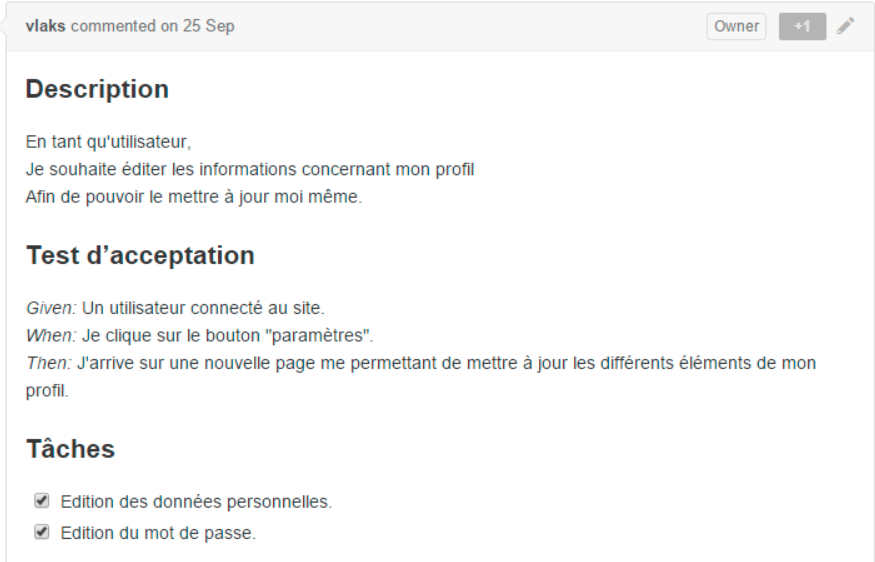
\includegraphics[width=6.3cm]{images/Process/accept-tests.png}
			\caption{\scriptsize Exemple de test d'acceptation}
			\label{fig:accept-tests}
		\end{wrapfigure}	
		\begin{minipage}{5cm}
			\begin{textblock}{6}(2.75,7)
			\begin{itemize}
				\item Tests d'intégration
				\item Tests d'acceptation
			\end{itemize}
			\end{textblock}
		\end{minipage}
\end{frame}


%\subsection{Qualification}
%\begin{frame}{Qualification}
%	\begin{itemize}
%		\item Déploiement continue de la branche master sur Heroku
%	\end{itemize}
%\end{frame}
